\label{\documentclass[conference]{IEEEtran}
\IEEEoverridecommandlockouts
% The preceding line is only needed to identify funding in the first footnote. If that is unneeded, please comment it out.
%\usepackage{cite}
\usepackage{amsmath,amssymb,amsfonts}
\usepackage{algorithmic}
\usepackage{graphicx}
\usepackage{textcomp}
\usepackage{xcolor}

%自定义宏包
	\usepackage{graphicx}
	\usepackage{amsmath,amsthm}
	\usepackage{amssymb,amsfonts}
	
	
	\usepackage{float} %指定图片位置
	\usepackage{subfigure}%并排子图 共享标题 有子标题
	\usepackage{caption}
	
	\usepackage{hyperref}

%算法宏包
	\usepackage[linesnumbered,ruled,vlined]{algorithm2e}
%\usepackage{setspace}

%导入文献
	\usepackage[backend=bibtex,sorting=none]{biblatex}
	\addbibresource{ref.bib}







\def\BibTeX{{\rm B\kern-.05em{\sc i\kern-.025em b}\kern-.08em
    T\kern-.1667em\lower.7ex\hbox{E}\kern-.125emX}}


\begin{document}

\title{Conference Paper Title*\\
%{\footnotesize \textsuperscript{*}Note: Sub-titles are not captured in Xplore and should not be used}
%\thanks{Identify applicable funding agency here. If none, delete this.}
}

\author{\IEEEauthorblockN{ Han Li}
	\IEEEauthorblockA{\textit{\footnotesize School of Information Science and Engineering} \\
		\textit{Yunnan University}\\
		Kunming,China \\
		lihan@mail.ynu.edu.cn}
	\and
	\IEEEauthorblockN{ Weidong Li}
	\IEEEauthorblockA{\textit{\footnotesize School of Mathematics and Statistics} \\
		\textit{Yunnan University}\\
		Kunming,China \\
		weidongmath@126.com}
	\and
	\IEEEauthorblockN{Xuejie Zhang*}
	\IEEEauthorblockA{\textit{\footnotesize School of Information Science and Engineering} \\
		\textit{Yunnan University}\\
		Kunming,China \\
		xjzhang@ynu.edu.cn}
}

\maketitle

\begin{abstract}
	%自然现象是所有启发式算法的来源, 例如, 粒子群算法(PSO)是一种模仿群体觅食行为发展起来的一种启发式算法, 粒子群算法来源于群体的觅食行为. 然而, 许多启发式算法只能解决连续的问题, 对于离散的问题, 没有很好的解决的方法, 这就严重限制了这些算法在实际工程问题中的使用,或多或少都模仿了梯度 因为离散的决策变量都有着实际的物理意义, 在本文中, 我们借鉴了基因算法和模拟退火算法, 根据问题的物理背景,改进了侏儒猫鼬算法使它能够解决物理问题
	%与物理系统退火过程的相似
	Natural phenomena are the source of all heuristic algorithms.
	For example, particle swarm optimization(PSO) algorithm comes from the foraging behavior of population~\cite{psofirst}. 
	The dwarf mongoose optimization algorithm (DMO) simulates the foraging behavior of the dwarf mongoose. 
	Simulated annealing algorithms (SA) is very similar to the physical system annealing process~\cite{sa_first}.
	However, many heuristic algorithms can only solve continuous problems, because them more or less imitated gradient. For discrete problems, there is no good solution, which severely limits the use of these algorithms in practical engineering problems. Because discrete decision variables have practical physical significance.
	In this paper, we use genetic algorithms (GA) and simulated annealing algorithms for reference, and improve the dwarf mongoose optimization algorithm according to the physical background of the problem to enable it to solve physical problems
\end{abstract}

\begin{IEEEkeywords}
component, formatting, style, styling, insert
\end{IEEEkeywords}

\section{Introduction}
This document is a model and instructions for \LaTeX.
Please observe the conference page limits. 

% 侏儒猫鼬算法简介
\section{An introduction to Dwarf Mongoose Optimization Algorithm}
%这是非洲的一种食肉动物, 分工
	The DMO algorithm is inspired by unique compensatory behavioral adaptations of the dwarf mongoose~\cite{dmo_first}. Dwarf mongoose is a carnivore in African, although this animal is small in size. They perform foraging and other behaviors through division of labor, so they engage in many compensatory behaviors. 
	
%不同于人类是父权制社会, 侏儒猫鼬是母权制的社会. 并不是雌性来照看幼崽, 通常是选择一定数量的个体来当保姆
	Unlike humans, which are a patriarchal society, dwarf mongoose are a matriarchal society. It is not the female that takes care of the pups, but usually a certain number of individuals are selected to act as babysitters. 
	
%算法将种群分为三个组, 当a进行觅食时, 
%The optimization starts with the alpha group setting out (exploring space) foraging, leaving the babysitters and the young at the nest.
%
	The algorithm divide the population into three groups: the alpha
	group, babysitters, and the scout group. When the alpha group go out to look for food, the young and babysitters stay at the nest. Note that looking for food means exploring space.
	
\subsection{Babysitters}
	The babysitters don't go out foraging, they stay with the young. To be fair, babysitters are rotated periodically, and other individuals in the population assume the role of babysitters.
	and the number of them depends on the the number of individuals. In our experiments, we set the number of nannies to $3\%$. 

\subsection{Alpha group}
	The number of individuals in the population is $n$, $X^{t}$ denotes all individuals in the population at time $t$, $X^{t}_{i}$ represents the $i$th individual in the population at that time. In every iteration, the probability value for each population which is select as a alpha female is calculated is as follows:
\begin{equation}
	\alpha=\frac{f ^{t}_i}{\sum_{i=1}^n f ^{t}_i}
	\label{choosepeep}
\end{equation}
	And the alpha group is updated in the following way:
\begin{equation}
	X^{t+1}=X^t+ phi * \text { peep }
	\label{upx}
\end{equation}
where, $phi$ follows a uniform distribution $phi\sim U[-1, 1]$.
	In every iteration, the sleeping mound is calculated as the Equation~\ref{sm}, and the average value of the sleeping mound is calculated as the Equation~\ref{phi}.
\begin{equation}
	s m ^ t _i=\frac{f^{t+1}_i - f^t_ i}{\max \left\{\left|f^{t+1} , f^t_ i\right|\right\}}
	\label{sm}
\end{equation}	
\begin{equation}
	\varphi=\frac{\sum_{i=1}^n s m_i}{n}
	\label{phi}
\end{equation}

\subsection{Scout group}
	The scouts find the next sleeping mound, and the mongooses do not come back to previous sleeping mound, which can ensure no overgrazing. In other words, this behavior ensures exploration validity. Equation~\ref{scout} imitated this behavior. 
\begin{equation}
	X_{i}^{t+1}=
	\begin{cases}
		X_i^t-C F * \text { phi } * \text { rand }
		*\left[X_i^t-\overrightarrow{\boldsymbol{M}}\right], \\
		\quad\quad\quad\quad\quad\quad\quad\quad \text { if } \varphi_{i+1}>\varphi_i \\
		X_i^t+C F * \text { phi } * \text { rand* 		
		}\left[X_i^t-\overrightarrow{\boldsymbol{M}}\right], \\
		\quad\quad\quad\quad\quad\quad\quad\quad \text { else }
	\end{cases}
\label{scout}
\end{equation}
	where, $rand$ is a random number between $0$ and 1, $CF$ is the parameter which can controls
	the collective-volitive movement of the mongoose and is calculated in Equation~\ref{cf}. And $\overrightarrow{\boldsymbol{M}}=\sum_{i=1}^n \frac{X_i \times s m_i}{X_i}$.
\begin{equation}
	 C F=\left(1-\frac{i t e r}{M a x_{i t e r}}\right)^{\left(2 \frac{i \text { iter }}{M a x_{i t e r}}\right)}
	 \label{cf}
\end{equation}

\subsection{Description of DMO algorithm}
%流程图如图所示, 当初始化和计算出适应度, 下一步是选择下一步是选择保姆, 他们不参与觅食.
	The flow chart of this algorithm is shown in Figure~\ref{flow_dmo}. When a population is initialized, the algorithm begins. When the number of iterations is less than the maximum number of iterations, calculating the fitness. And next step is to choose babysitters, who are not involved in foraging. Then perform update of alpha group. All but babysitters in the population were updated. At the time of renewal, a female was first selected using Equation~\ref{choosepeep}, and using Equation~\ref{upx} to update this individual. We need to calculate sleep mound and the average of the sleep mound in order for scouts group to use. The final step of alpha group is setting the time counter $C$. 
	
%图片_侏儒猫鼬算法流程图
\begin{figure}[t]
	%居中
	\centering
	%\includegraphics[width=2.5in]{Autoencoder1}
	%占据0.8宽度
	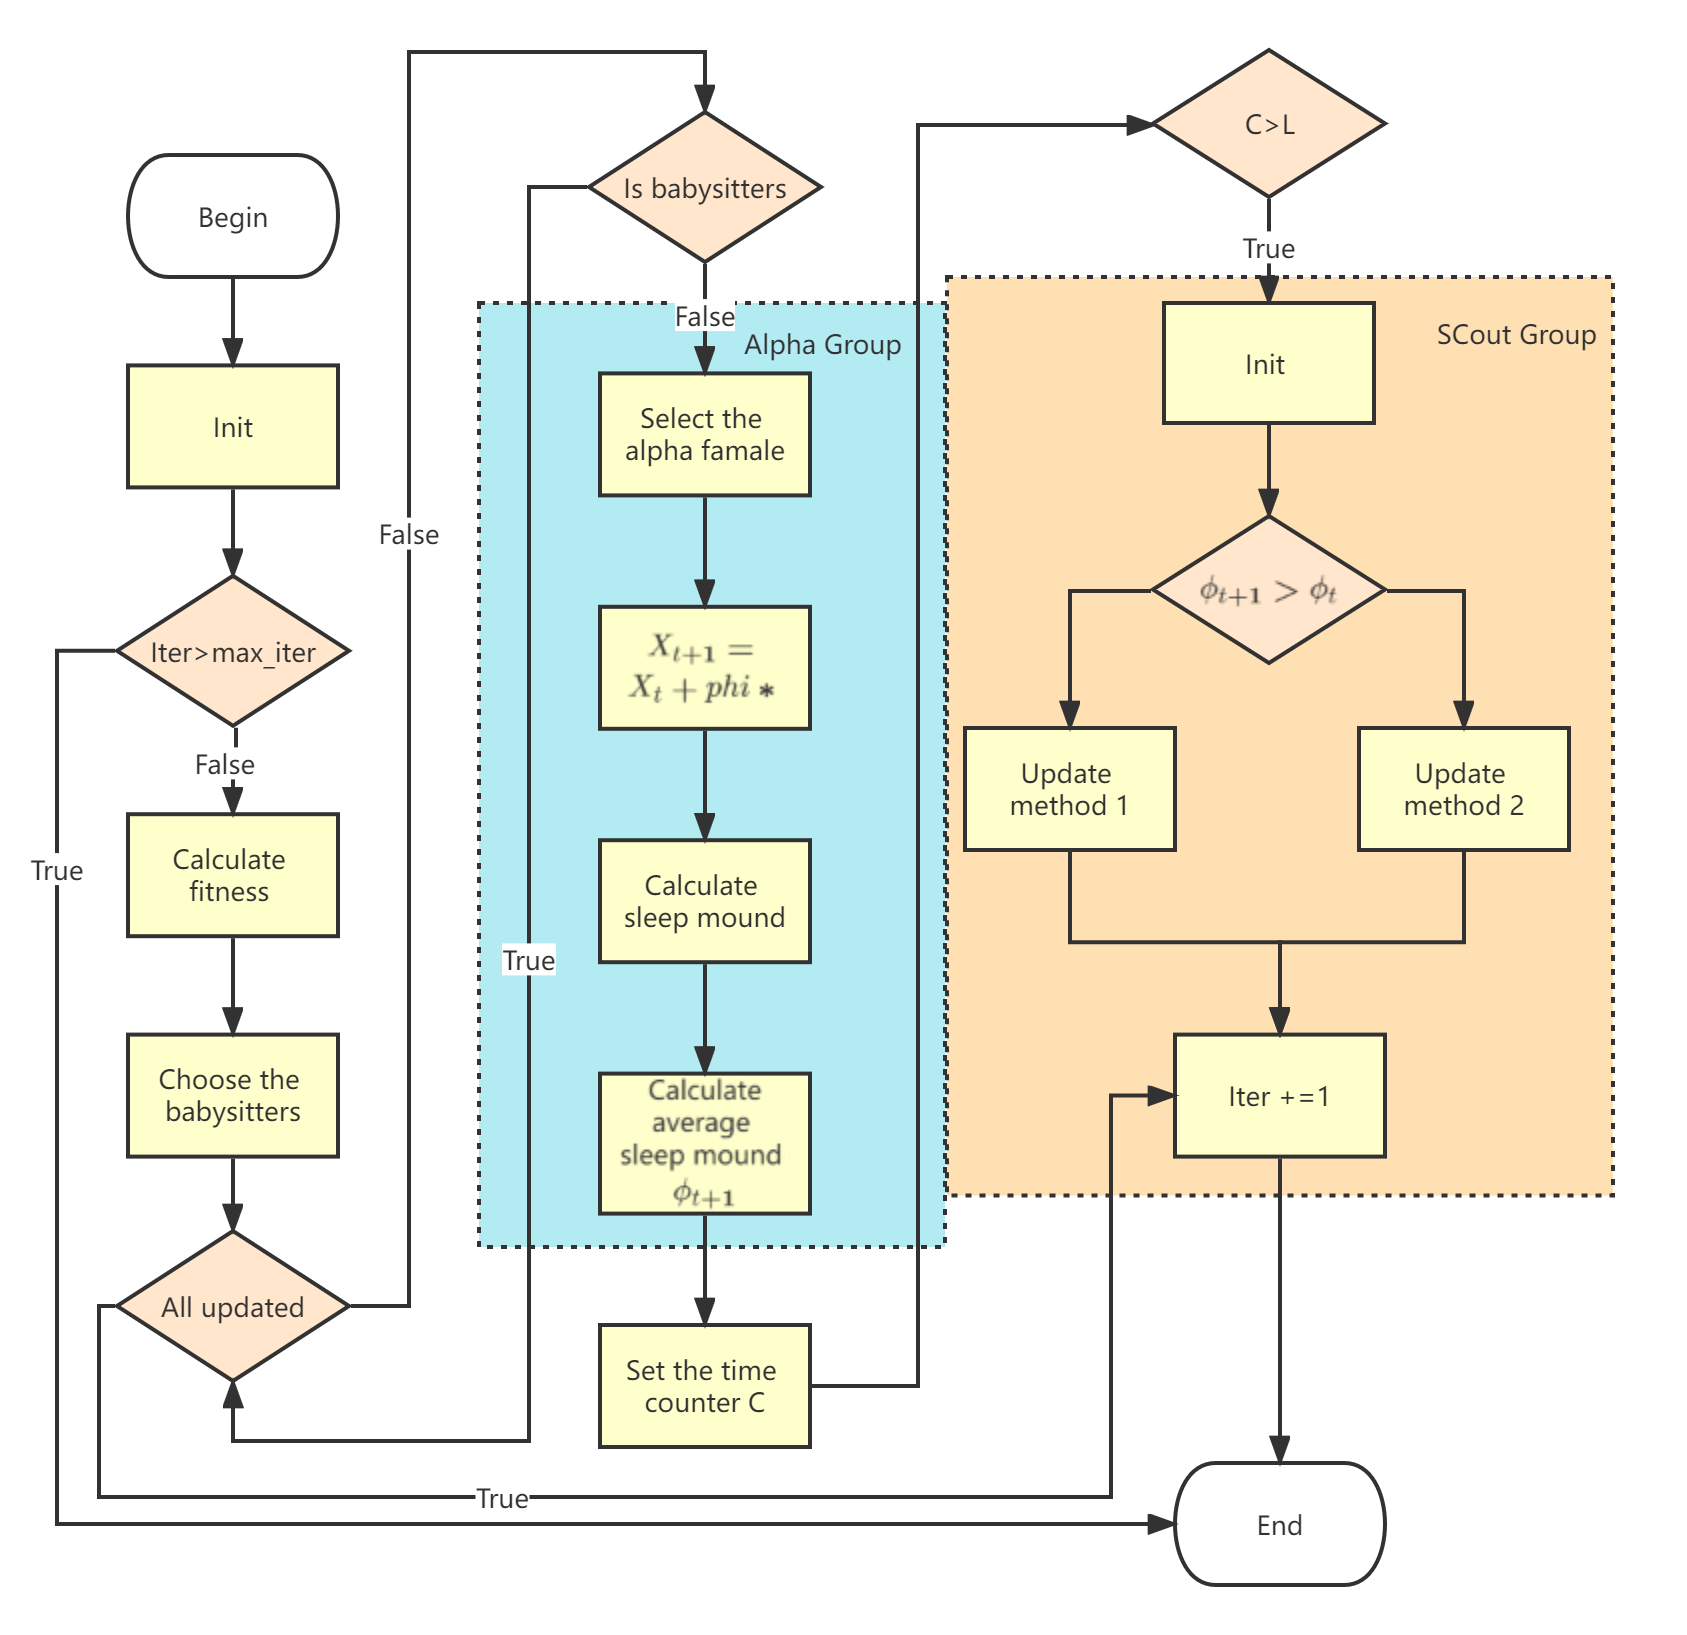
\includegraphics[width=0.50\textwidth]{flow_dmo.png}
	%图片名称
	\caption{Flow chart of genetic algorithm}
	\label{flow_dmo}
\end{figure}






\section{Discrete Dwarf Mongoose Optimization Algorithm}
%我们将用两种方式描述并行机问题, 以便于更好的理解决策变量的表示形式
	The key step in designing a discrete algorithm is to define the representation of the solution. Because each decision variable has a real physical meaning. 
	
%在设计更新操作时, 我们借鉴了基因算法的更新方法
	In designing the update operation, we use the update method of genetic algorithm for reference.
	The GA which is based on Darwin's theory of natural selection which is published by John Holland in \citeyear{gafirst}~\cite{gafirst} is a smart heuristic algorithm that can be used to solve integer programming. However, the genetic algorithm does not consider the actual physical meaning of the decision variables, but only encodes variables to solve discrete problems. it draws on the behavior of chromosomes in cells.
	In Darwin's theory of natural selection, individuals adapted to the environment survive and reproduce. % chromosome 染色体
	In the process of biological reproduction, chromosome experience crossover and mutation.
	%it simulates the process of natural selection and reproduction to solve optimization problems. 
	Because GA need to simulate the behavior of chromosomes, we need to encode and decode every iteration which requires a lot of calculation, as shown in Figure~\ref{flowga}. 
%基因算法是一种基于自然选择学说的优化算法被张三于1000年提出, 同时借鉴了细胞中染色体的行为
%图片_基因算法流程图
\begin{figure}[htbp]
	%居中
	\centering
	%\includegraphics[width=2.5in]{Autoencoder1}
	%占据0.8宽度
	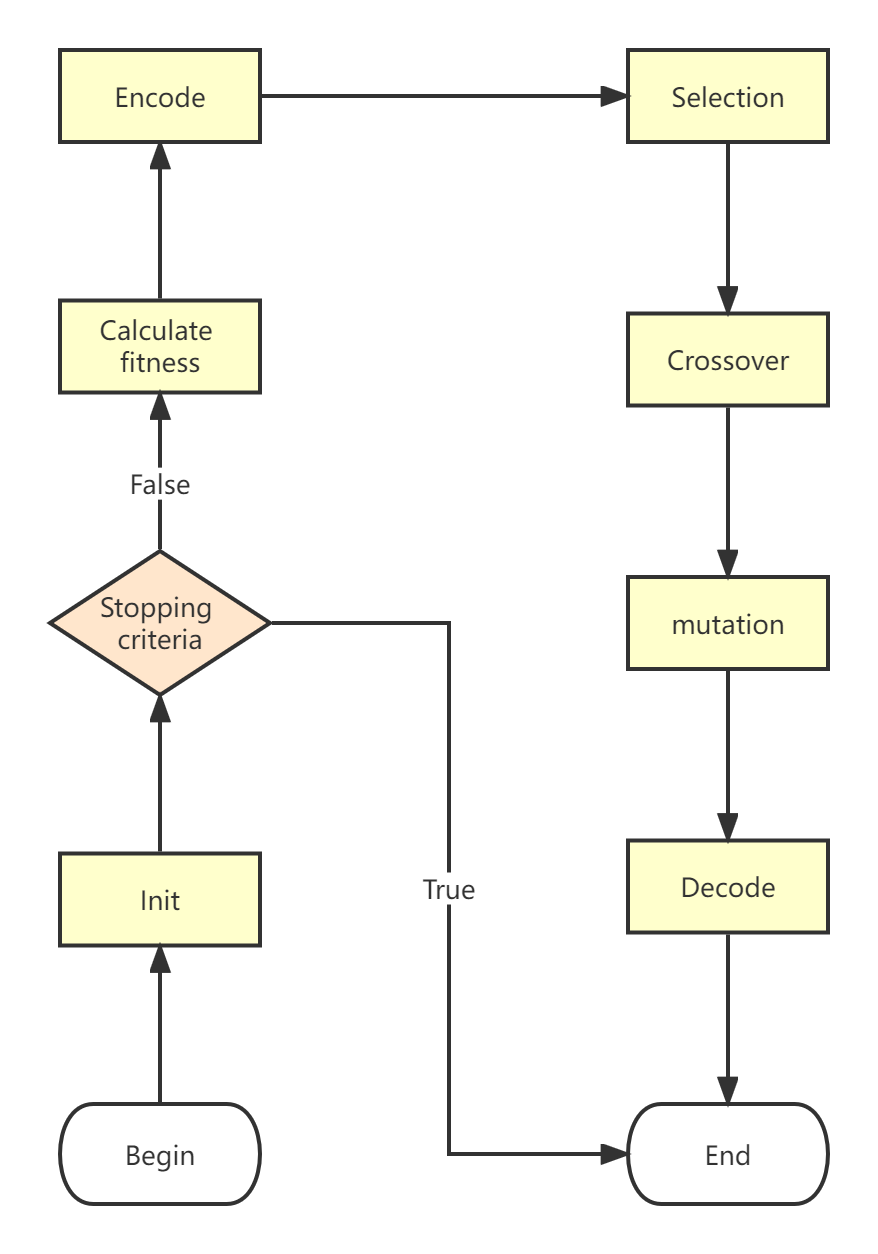
\includegraphics[width=0.30\textwidth]{flow_ga_2.png}
	%图片名称
	\caption{Flow chart of genetic algorithm}
	\label{flowga}
\end{figure}	

%图片_基因算法编码
\begin{figure}[htbp]
	%居中
	\centering
	%\includegraphics[width=2.5in]{Autoencoder1}
	%占据0.8宽度
	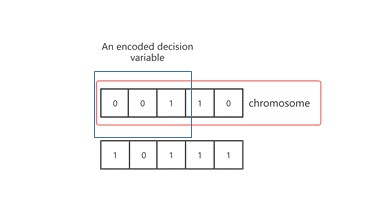
\includegraphics[width=0.40\textwidth]{ga_ch.jpg}
	%图片名称
	\caption{Coding operations in GA}
	\label{ga_ch}
\end{figure}
%当进行编码时, 编码的位数由上界, 下界, 以及间隔决定.公式如下
	When encoding the variable, the number of bits encoded is determined by the upper bound, the lower bound, and the interval. The formula is as follows:
\begin{equation}
	m= \lceil \log _2 \frac{ub-lb}{p}+1  \rceil
\end{equation}
Where $ub$ is the upper bound, $lb$ is the lower bound, and $p$ is the interval.

%就像是在图片中展示, 在基因算法中, 前三位是一个决策变量, 
As shown in the Figure~\ref{ga_ch}, in genetic algorithm, the first three binary digits form a decision variable.
%当进行变量的更新时, 只需要对编码后的串进行类似于逻辑运算一样的操作
When updating a variable , only the encoded string needs to be operated like a logical operation.

Ternary Operators($a * X_1 - X_2$)


	
	
	
	
	
	
	
	Our problem is homogeneous with the parallel machines scheduling problem. We will describe the  problem in two ways, in order to better understand the representation of the decision variables.
	

\subsection{The Parallel Machines Scheduling Problem}
	
	The description of it is as follows: there are $n$ jobs $J =\{1, \dots, n\} $, $m$ machines which are identical $M = \{1, \dots, m\}$. Each job $j$ is independent. 
	Every job should be finished on one of that machines, and the time which the job $i$ need on the machine for processing job is $p_i$.
	Once the jobs are placed on the machine, they need to work until it is completed. As a result, they can not be interrupted.
	Such that the maximum running time of all machines is minimized.
	
	The parallel machines scheduling problem can be formulated as an integer programming problem:
\begin{align}
	\min& \max \limits _ {1 \le j \le m}\sum_{i=1}^n p_i x_{i j} \label{pmpmin1} \\
	\text{s.t.} 
	&\sum_{j=1}^m x_{i j}=1 \quad i=1, \ldots, n  \label{pmpst1} \\
	& \quad x_{ij} \in\{0,1\}                   \label{pmpst2}
\end{align}
	Where the Equation~(\ref{pmpmin1}) shows that we should minimize the maximum completion time. The Equation~(\ref{pmpst1}) shows each job must be assigned to a machine. If $x_{ij} = 1$, it means that job $i$ is assigned to $j$'s machine. 

	However, the spatial complexity of this formulation is $ O(mn) $, and because each variable is a binary variable, so the time complexity is $ O(2^{mn} ) $. We formulate the parallel machines scheduling as another form.
\begin{align}
	\min& \max \limits _ {1 \le j \le m}   \sum\limits_{1\le i \le n, x_i = j} p_i \label{pmpmin2} \\
	\text{s.t.} 
	%&\sum_{j=1}^m x_{i j}=1 \quad i=1, \ldots, n  \label{pmpst1_1} \\
	& \quad x_{i} \in\{0,1,\dots, m\} , \quad i=1, \ldots, n
\end{align}
	Where the spatial complexity of this formulation is $ O(n) $, and the time complexity is $ O(m^n ) $





\begin{algorithm}[t]
%设置算法编号
%\renewcommand{\thealgocf}{3-1}
\SetAlgoLined %显示end
\caption{Discrete Dwarf Mongoose Optimization Algorithm}%算法名字
\label{}% 标签
\KwIn{Parameters $ n$}%输入参数
\KwOut{Best solution}%输出
	%-----------------begin here----------------
	%      '\;'   用于换行
	Initialize the algorithm parameters:[peep] \\
	Initialize the mongoose populations (search agents): $n$  \\
	Initialize the number of babysitters: $bs$  \\
	% Set $n=n-bs$  \\
	Set babysitter exchange parameter $L$
	
	\For{iter = 1 : m }{
		\For{k = 1 : bs}{
			Select the babysitters \\
		}
		Calculate the fitness of the mongoose \\
		Set time counter $C$ \\
		Find the alpha based on the equation:
		$\alpha=\frac{f i t_i}{\sum_{i=1}^n f i t_i}$ \\
		Produce a candidate food position based on the equation: 
		$$X^{t+1}_{i}=p h i *[X^{t}_i + X^{t}_{ peep }]$$ \\
		Evaluate new fitness of $X_{i+\mathbf{1}}$  \\
		Evaluate sleeping mound
		$$s m_i=\frac{|f i t_{i+1}-f i t_i|}{\max \left\{\left|f i t_{i+1}, f i t_i\right|\right\}}$$    \\
		Compute the average value of the sleeping mound found:
		$$\varphi=\frac{\sum_{i=1}^n s m_i}{n}$$ \\
		Compute the movement vector using 
		$$\overrightarrow{M}=X_{cbest}$$  \\
		Exchange babysitters if $C \geq L$, and set initialize bs position and calculate fitness 
		$f i t_i \leq \alpha$ \\
		Simulate the scout mongoose next position using
		\begin{equation*}
			X_{i+1}=
			\begin{cases}
				%case1
				(C F * phi * rand)*[X_i+\overrightarrow{M}]\\
				%
				\quad\quad\quad\quad\quad\quad\quad\quad \text { if } \varphi_{i+1}>\varphi_i \\
				(C F * phi * rand)*[ \overrightarrow{M}+ X_i ]\\
				\quad\quad\quad\quad\quad\quad\quad\quad \text { else }
			\end{cases}
		\end{equation*}
	}%for
	return best solution
\end{algorithm} 




\subsection{Different From GA}






\subsection{Our Algorithm}
	In our algorithm, we learned from Mendel's genetic law. We define the decision variables of individuals with higher fitness as dominant traits.
	In Mendel's experiment, the first generation of tall and short stemmed peas produced offspring with tall stems. Similarly, we define that dominant traits cover hidden traits.

%我们定义了一个三元运算符, x是一个控制变化的数字, y是两个维度相同的向量, 首先我们计算
	We define a ternary operator ($p h i *[X_a + X_{ b }]$), $phi \in (0, 1)$ is a number that controls the variation, and $X_a, X_b$ are two vectors of the same dimension. At first, we compute $X_c = p h i * X_a + (1-phi) * X_b$, for each element in X, the probability of being selected is calculated by the following formula:
\begin{align}
	&  X_c= p h i * X_a + (1-phi) * X_b \\
	& p(X_{ai}) = \frac{|X_{bi}- X_{ci}|}{|X_{bi} - X_{ai}|} 
\end{align} 
	

\section{}





\section{Prepare Your Paper Before Styling}
Before you begin to format your paper, first write and save the content as a 
separate text file. Complete all content and organizational editing before 
formatting. Please note sections \ref{AA}--\ref{SCM} below for more information on 
proofreading, spelling and grammar.

Keep your text and graphic files separate until after the text has been 
formatted and styled. Do not number text heads---{\LaTeX} will do that 
for you.


\section*{Acknowledgment}

The preferred spelling of the word ``acknowledgment'' in America is without 
an ``e'' after the ``g''. Avoid the stilted expression ``one of us (R. B. 
G.) thanks $\ldots$''. Instead, try ``R. B. G. thanks$\ldots$''. Put sponsor 
acknowledgments in the unnumbered footnote on the first page.

% \printbibliography



\end{document}
}